% The landing stack and its three test beds (TikZ; every label is defined in Section 3).
\begin{figure*}[t]\centering
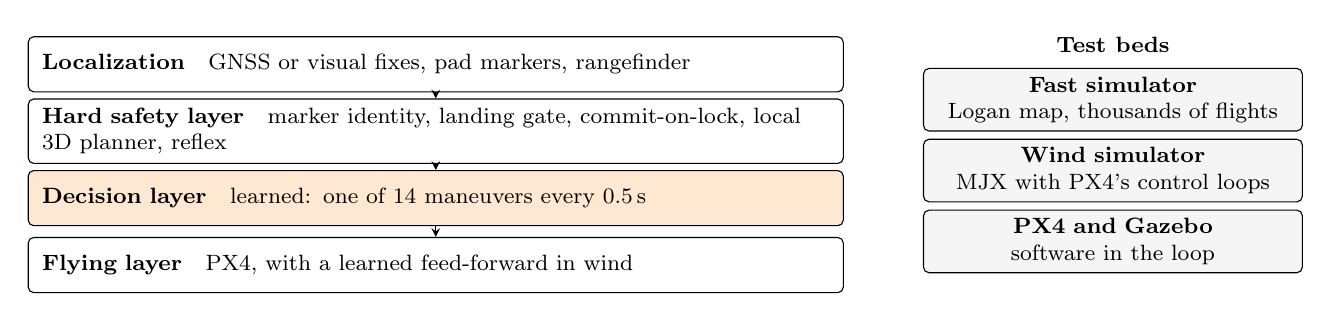
\begin{tikzpicture}[font=\footnotesize, >=stealth,
  layer/.style={draw, rounded corners=2pt, text width=10.0cm, minimum height=7mm, align=left, inner xsep=5pt},
  bed/.style={draw, rounded corners=2pt, text width=4.6cm, minimum height=7mm, align=center, fill=black!4, inner sep=3pt}]
  \node[layer] (loc)  at (0, 0)     {\textbf{Localization}\hspace{1em}GNSS or visual fixes, pad markers, rangefinder};
  \node[layer] (safe) at (0, -0.85) {\textbf{Hard safety layer}\hspace{1em}marker identity, landing gate, commit-on-lock, local 3D planner, reflex};
  \node[layer, fill=orange!18] (dec) at (0, -1.7) {\textbf{Decision layer}\hspace{1em}learned: one of 14 maneuvers every 0.5\,s};
  \node[layer] (fly)  at (0, -2.55) {\textbf{Flying layer}\hspace{1em}PX4, with a learned feed-forward in wind};
  \foreach \a/\b in {loc/safe, safe/dec, dec/fly} \draw[->] (\a.south) -- (\b.north);
  \node[bed] (fast) at (8.6, -0.45) {\textbf{Fast simulator}\\ Logan map, thousands of flights};
  \node[bed] (mjx)  at (8.6, -1.35)  {\textbf{Wind simulator}\\ MJX with PX4's control loops};
  \node[bed] (gz)   at (8.6, -2.25) {\textbf{PX4 and Gazebo}\\ software in the loop};
  \node[font=\footnotesize\bfseries] at (8.6, 0.25) {Test beds};
\end{tikzpicture}
\caption{The landing stack: four layers, one learned decision layer, and the three test beds that run it.}\label{fig:stack}
\end{figure*}
